%\section{Discussion}


\subsection{Comparison of beading schemes}
We can see from \cref{TEST_naive_accuracy}(top) and~\ref{over_underfill} that the uniform technique causes a lot of overfills and underfills: on average approximately \SI{1}{\percent} of the total target area is covered by underfill and likewise for overfill.
To our knowledge, the uniform beading scheme, as well as the outer beading scheme, is of little use to FDM printers.

The constant bead count scheme effectively deals with underfills, but generates orders of magnitude more overfills compared to the other schemes. 
Also, the scheme comes at the cost of greatly varying bead widths and an average bead width that is not close to the preferred bead width.
Note that most overfill areas occur near regions of alternating bead width. 
For an input outline shape which contains both very small and very large features, the constant bead count scheme produces bead widths which can fall outside of the range of manufacturable bead widths.
Moreover the centrality marking is not robust against small perturbations in the outline; adding a small chamfer in a corner causes the unmarked ST to be very small at that location, which results in tiny bead widths.

In \cref{TEST_Center_accuracy} we can see that
the centered beading scheme effectively deals with both overfill and underfill and produces desired bead widths in all locations, except for the extrusion paths in the center, where the bead widths \revise{are within a factor 2 off from the desired bead width.}{range between $0.5 w^*$ and $1.8w^*$, i.e. the deviation is within a factor of $3.2$.}
According to \cref{over_underfill} the overfill and underfill for the centered, the evenly distributed and the inward distributed scheme are all approximately \SI{0.2}{\percent}, which is a considerable improvement over the uniform technique.

However, according to \cref{widthHistogram} the centered scheme exhibits a wider range of bead widths than the distributed schemes:
the standard deviation of the bead widths in the centered scheme is approximately \SI{39}{\micro\meter}, while that of the distributed schemes is approximately \SI{14}{\micro\meter}.
\revise{}{Moreover, because the quantization operator rounds to the nearest number of beads the bead widths range from $0.75w^*$ to $1.5w^*$, i.e. the deviation is within a factor $2$, which is considerably lower than in the centered scheme.}
We therefore conclude that the distributed schemes \revise{result in bead widths closer to the preferred widths}{exhibit a lower bead width deviation} compared to the centered scheme.
%This is desirable for the manufacturability of the beads and can therefore have a positive effect on the mechanical properties and surface quality of the 3D prints. 

It is hard to visually identify the difference between the evenly and the inward distributed scheme in \cref{visualized_accuracy}, because that particular example shape does not have wide features.
However, \cref{distributed_comparison} and  \cref{widthIndexedHistogram} confirm that the outer toolpaths have the preferred bead width more often.
Furthermore, from \cref{smoothness} we find that compared to evenly distributed, the inward distributed scheme produces smoother toolpaths overall.
Thus the inward distributed scheme prevents over- and underfill, generates smooth toolpaths with more homogeneous width and affects smaller more centered parts of the print than the other schemes. 






\subsection{Applications}
Toolpath with varying width is particularly meaningful for narrow parts, since there the negative effect of under- and overfill is more pronounced than in wide parts.
In extreme cases, thin features will not be filled at all.
Therefore, our framework, while working for wide parts as well, shows most of its potential for objects which contain thin parts.

\Cref{applications_overview} collectively shows the application of the proposed inward distributed scheme for various types of 3D model, including both thin parts (architectural models, casings, embossed text, gears and microstructures) and wide parts (\cref{applications_case}) and organic shapes (\cref{applications_statue})).

For architectural models and casings, preventing over- and underfill is expected to make them stronger. 
For embossed text, preventing underfill reduces the various holes in the top surfaces, which is detrimental to the visual quality of those top surfaces.
For gears and similar mechanical parts that are designed with finite element analysis, the less variation in extrusion widths is closer to the assumptions under fast analysis (e.g. using homogenization~\cite{Liu2016CAD}).

Of particular interest are microstructures that could be uniquely fabricated by 3D printing.
For example, topology optimized bone-like structures~\cite{wu2017infill} contain filaments of varying thickness that follow a varying stress direction (\cref{applications_bone}).
An angled Gyroid structure with uniform thickness also results in outline shapes with varying width (\cref{applications_gyroid}). 
These structures are accurately densely filled using our framework.
Another class of microstructures consists of parameterized patterns with varying thickness to achieve functional gradation.
\Cref{applications_hex} shows the contour-parallel toolpath with varying width of a hexagonal grid neatly switches between different bead counts over the volume, preventing the jagged moves a direction-parallel toolpath would create for such a case~\cite{bates2018compressive}.


\begin{figure*}
\centering
\setlength{\figwidth}{0.099\textwidth}
\setlength{\figheight}{0.099\textwidth}
\begin{subfigure}{\textwidth}\centering
\censorbox{
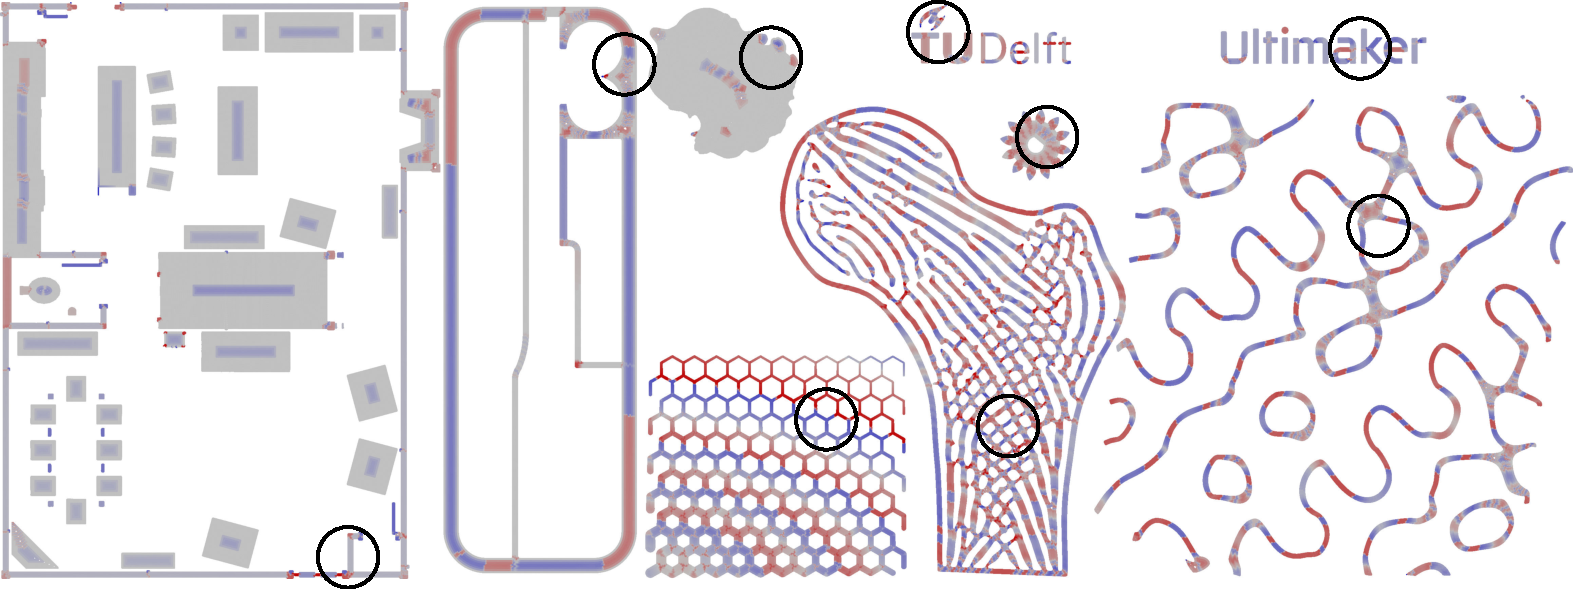
\includegraphics[width=\textwidth]{sources-applications-combined-small-dilated-circled.pdf}
}
%\caption{Overview}\label{applications_overview}
\end{subfigure}
\begin{subfigure}[t]{\figwidth}\centering
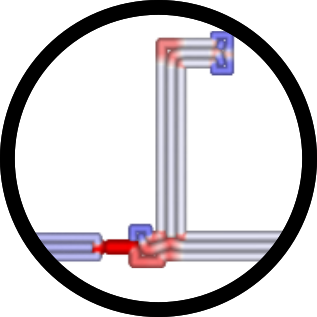
\includegraphics[height=\figheight]{sources-applications-house.png}
\caption{House}\label{applications_house}
\end{subfigure}
\begin{subfigure}[t]{\figwidth}\centering
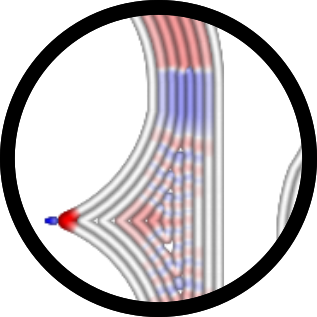
\includegraphics[height=\figheight]{sources-applications-pocket-operator-case.png}
\caption{Case}\label{applications_case}
\end{subfigure}
\begin{subfigure}[t]{\figwidth}\centering
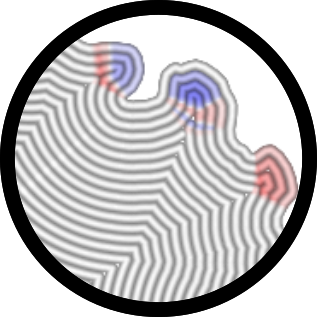
\includegraphics[height=\figheight]{sources-applications-david.png}
\caption{Statue}\label{applications_statue}
\end{subfigure}
\begin{subfigure}[t]{\figwidth}\centering
\censorbox{
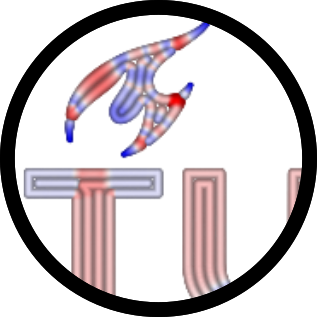
\includegraphics[height=\figheight]{sources-applications-tud-logo.png}
}
\caption{\censor{TUD}}\label{applications_tud}
\end{subfigure}
\begin{subfigure}[t]{\figwidth}\centering
\censorbox{

\includegraphics[height=\figheight]{sources-applications-ultimaker-logo.png}
}
\caption{\censor{UM}}\label{applications_um}
\end{subfigure}
\begin{subfigure}[t]{\figwidth}\centering
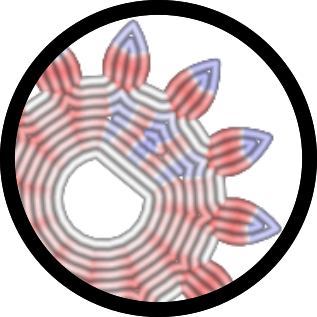
\includegraphics[height=\figheight]{sources-applications-pinion-gear-motor.png}
\caption{Gear}\label{applications_gear}
\end{subfigure}
\begin{subfigure}[t]{\figwidth}\centering
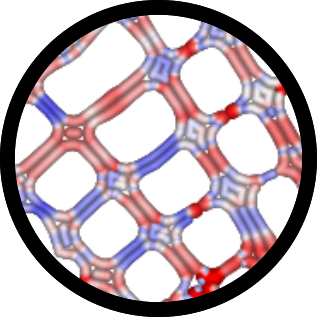
\includegraphics[height=\figheight]{sources-applications-topopt-bone.png}
\caption{Bone}\label{applications_bone}
\end{subfigure}
\begin{subfigure}[t]{\figwidth}\centering
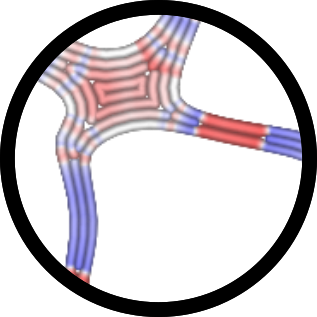
\includegraphics[height=\figheight]{sources-applications-gyroid.png}
\caption{Gyroid}\label{applications_gyroid}
\end{subfigure}
\begin{subfigure}[t]{\figwidth}\centering
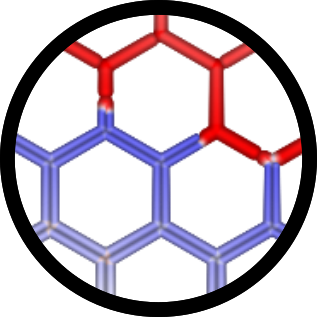
\includegraphics[height=\figheight]{sources-applications-hex-grid.png}
\caption{Hex}\label{applications_hex}
\end{subfigure}
\begin{subfigure}[t]{.3\figwidth}
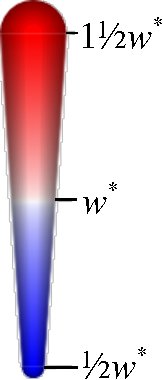
\includegraphics[height=\figheight]{sources-validation-widths-legend-small.pdf}
\end{subfigure}
\caption{
Visualization of the widths for the output toolpaths of the inward distributed beading scheme {($N=3$) }applied to various example application objects.
From left to right and top to bottom: a house, a case for electronics, a statue, two common logos, a gear, a topologically optimized bone structure, a tilted homogeneous gyroid structure and a heterogeneous thickness hexagonal grid.
}
\label{applications_overview}
\end{figure*}












\subsection{Discussion on implications}
Note that the current industry standard in FDM printing employs little to no bead width variation.
Properly performing bead width variation calls for adaptations and developments in printers and firmware.
In the beading schemes we set a transition length of $t(n) = w^*$.
That will demand changes in cross-sectional area of the bead up to \SI{200}{\percent} over a small distance that is comparable to the nozzle size, which is challenging for some hardware systems.
Varying the movement speed can be utilized to change the cross-sectional area, but this approach is limited, since the movement speed is constrained by acceleration considerations near bends in the toolpath~\cite{Ertay2018,Kuipers2018}.
Our schemes require a more accurate control of the volumetric flow rate in \si{\milli\meter\cubed\per\second}.
Using a filament feeder directly mounted on the print head (a.k.a. direct drive) can control the flow more dynamicaly then FDM printers where the material is fed through a Bowden tube from a feeder mounted on the frame.
Still direct drive printers require some control system in order to accurately change the volumetric flow rate such as pressure advance algorithms~\cite{tronvoll2019investigating}.
Yet inaccuracies in direct drive systems employing advance algorithms might arise due to the changes in back-pressure required by changing bead size.
We expect that developments in printing hardware and firmware will address these challenges in the future.


Another limiting factor for adopting adaptive bead width is the format of G-code which stores machine instructions.
G-code does not support moves with varying cross-sectional area.
A typical extrusion move \lstinline{G1 X$x$ Y$y$ E$v$} only specifies the total amount of volume $v$ to be extruded in the move, not how that total amount should be distributed along the extrusion move.
A workaround is to approximate a variable width extrusion segment by smaller segments with constant width.
However, this introduces errors nevertheless.
Ideally the G-code language would be expanded in some way to allow for extrusion segments with varying cross-sectional area.


% Taking a broader perspective, we note that our proposed inward distributed scheme is a pragmatic solution.
% Rather than deriving some optimal beading scheme from a clear specification of the objective, we propose some arbitrary inward distributed beading scheme and show that it is better than the other beading schemes.
% An optimal beading scheme can be derived if the objective is formalized terms of a unambiguous fitness function, but that would depend on the specific hardware setup and application for which toolpaths are generated.
% This manuscript is therefore limited to showing the flexibility and versatility of the framework, rather than deriving an optimal beading scheme.




